\documentclass[12pt]{article}
\usepackage[utf8]{inputenc}
\usepackage[english]{babel}
\usepackage{graphicx}
\usepackage{float}
\usepackage{amsmath}
\usepackage[table]{xcolor}
\usepackage{xcolor}
\usepackage{enumitem}
\usepackage{titlesec}
\usepackage{amssymb}
\usepackage{cancel}

\title{Homework 3}
\author{Leonard David Vivas Dallos \\ Mariana Valencia Cubillos \\ Samuel Mira Álvarez}
\date{October 8, 2023}

\begin{document}

\maketitle
\textbf{\textit{Assignment:}} Write solutions for following exercises/problems

\tableofcontents

\renewcommand{\thesubsection}{\thesection.\alph{subsection}}

\section{\textit{Plus-free and top-plus regular expressions}}

This problem considers two special classes of regular expressions.
\begin{itemize}
    \item A regular expression R is \textit{plus-free} is and only if never uses the $+$ operator.
    \item A regular expression R is \textit{top-plus} if and only if either
    \begin{itemize}
        \item $R$ is plus-free, or
        \item $R = S + T$, where $S$ and $T$ are top-plus.
    \end{itemize}
\end{itemize}
For example, $1((0^*10)^*1)^*0$ is plus-free and (therefor) top-plus; $01^*0+10^*1+\varepsilon$ is top-plus but not plus-free, and $0(0+1)^*(1+\varepsilon)$ is neither top-plus nor plus-free.
Recall that two regular expressions $R$ and $S$ are \textit{equivalent} if they describe exactly the same language: $L(R)=L(S)$.
\begin{enumerate}
[label=\alph*)]
    \item Prove that for any top-plus regular expressions $R$ and $S$, there is a top-plus regular expression that is equivalent to $RS$.
    \item Prove that for any top-plus regular expression $R$, there is a plus-free regular expression $S$ such that $R^*$ and $S^*$ are equivalent.
    \item Prove that for any regular expression $R$, there is an equivalent top-plus regular expression $S$.
\end{enumerate}
You may assume the following facts without proof, for all regular expressions $A, B,$ and $C$:
\begin{enumerate}
[label=\roman*)]
    \item $A(B+C)$ is equivalent to $B + AC$
    \item $(A+B)C$ is equivalent to $AC+BC$.
    \item $(A+B)^*$ is equivalent to $(A^*B^*)^*$.
\end{enumerate}

\subsection{Proof}

By induction the number $n$ of pluses in $R$ . We assume that for any $R$ with less than n pluses, there is a plus-free regular expression $S$ such that $R^*$ and $S^*$ are equivalent.

(Base Case) Let $n=0$ .
Then R is plus-free by definition and then $R^*$ is plus-free by definition.

(Induction Step) Let $n>0$.
Then $R$ has at least one plus. Thus, $R= R_1 +R_2$ where $R_1$ and $R_2$ are top-plus. Then, $R^*=(R_1+R_2)^*$
By the facts above we have, 
\begin{center}
    $(R_1+R_2)^* \equiv (R_1^*R_2^*)^*$
\end{center}
Now,  $R_1$ and $R_2$ have less than $n$ pluses. So, by induction hypothesis there are plus-free regular expressions  $S_1$ and $S_2$ such that $R_1^*$ and $S_1^*$ 
 and $R_2^*$ and $S_2^*$ are equivalent. Therefore, we can define $S=S_1^*S_2^*$ which is by definition plus-free and now $R^*$ and $S^*$ are equivalent.

 \subsection{Proof}

 Let $R$ be a regular expression. By induction the "size" of $R$ . We assume that for any  sub-expression $R$ , there is an equivalent top-plus regular expression $S$. Now, we have 5 cases based on which regular expression R is.
\begin{enumerate}
    \item $R=\emptyset$ 
Then, $R$ is plus-free and top-plus by definition.
\item $R = x$ , where x is a single string
Then, $R$ is plus-free and top-plus by definition.
    \item $R=R_1+R_2$ 
Then, we can use the induction hypothesis on $R_1$ and $R_2$. So, there are top-plus regular expressions  $S_1$ and $S_2$ such that $R_1$ and $S_1$ 
 and $R_2$ and $S_2$ are equivalent. Then $S= S_1 +S_2$ is a equivalent top-plus regular expression.
    \item $R=R_1R_2$
Then, we can use the induction hypothesis on $R_1$ and $R_2$. So, there are top-plus regular expressions  $T_1$ and $T_2$ such that $R_1$ and $T_1$ 
 and $R_2$ and $T_2$ are equivalent. Then $R=T_1T_2$ is a equivalent regular expression, and now we can use proof a) to affirm that there exists $S$ equivalent to $T_1T_2$ 
    \item $R=R_1^*$
By induction hypothesis we know that there is a top-plus regular expression $R_2$ that is equivalent to $R_1$. Then, $R$ is equivalent with $R_2^*$ . Now, by proof b) we can say that there is a plus-free regular expression $S_1$ such that $R_2^* \equiv S_1^* \equiv R^*$ and so, $S = S_1$. 
 \end{enumerate}
 

\section{\textit{Regular expression for a language}}
For the following language on $\sum = \{0,1\}^*$, determine a regular expression:

Strings $w$ in which the number of $0$s and the number of $1$s differ by a multiple of $3$.

\textit{Hint:} You may start with a DFA and then obtain an equivalent regular expression.

 \subsection{Proof}

We can construct a GNFA that simulates a automaton that accepts $w$ such that $|\#(0,w) - \#(1,w)| \equiv 0 \text{ mod } 3$. This automaton simulates a cycle of 3 states for which it  evaluates the current  $|\#(0,w) - \#(1,w)| \equiv 1, 2, 0 \text{ mod } 3$ . 

\begin{minipage}{\textwidth}
            \centering
            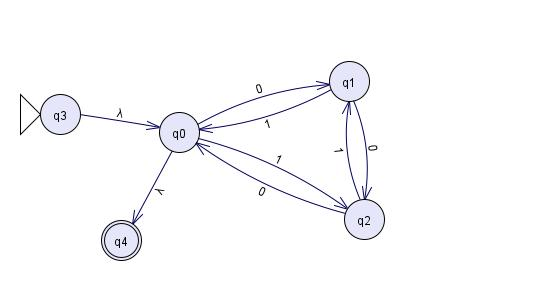
\includegraphics[width=0.75\textwidth]{Tarea 3 GNFA 2.a.jpg}
            \label{Enunciado Ej. 5}
        \end{minipage}

         It clearly accepts $\epsilon$ and all w such that $|\#(0,w) - \#(1,w)| \equiv 0 \text{ mod } 3$. 

         Then, we obtain an equivalent regular expression. So, the regular expression for the language that accepts strings $w$ in which the number of $0$s and the number of $1$s differ by a multiple of $3$ is:
\begin{equation*}
    ((1 \cup (00))(10)^*(0 \cup (11)) \cup (01))^*
\end{equation*}

\section{\textit{Proving non regularity}}
Let
\begin{equation*}
    L_{sqb}=\{w \in 1{0,1}^* | (w)_2 \text{ is a perfect square}\}
\end{equation*}
where $(w)_2$ denotes the integer with binary representation equal to the string $w$ (note that $w$ must have a leading $1$).

Prove that $L_{sqb}$ is not regular
\begin{enumerate}
[label=\alph*)]
    \item using the pumping lemma, and
    \item using the method of a witness set (fooling set)
\end{enumerate}

\subsection{Proof: Pumping Lemma}

Let $L_{sqb}$ the set described above. 
Assume (by contradiction) that $L_{sqb}$ is regular.
Let's see that if $\forall k\geq1, \exists w \in L, |w|\geq k, \forall x,y,z$, if
\begin{enumerate}
    \item $w=xyz$
    \item $|xy|\leq k$
    \item $y \neq \varepsilon$
\end{enumerate}
then
\begin{enumerate}
[start=4]
    \item $\exists l \geq 0$ such that $xy^lz \notin L$ 
\end{enumerate}

Let's notice that for $k \geq 2$, we have numbers of the form:
\begin{flalign*}
    (2^k+1)^2 &= 2^{2k}+2^{k+1}+1 \\
    &= (10^{k-2}10^k1)_2 \in L_{sqb}
\end{flalign*}
Let $w = 10^{k-2}10^k1 \in L_{sqb}$.
By pumping lemma, we can divide $w$ as follows $w=xyz$.

Taking $x=1, y=0^{k-2}$, it is clear that $|xy|=|10^{k-2}| \leq k$. Let's see that the string $xyyz \notin L_{sqb}$
\begin{flalign*}
    xyyz &= 10^{k-2}0^{k-2}10^k1 \\
    &= 10^{2k-4}10^k1
\end{flalign*}
Let's check what is the decimal representation of the string given above.
\begin{flalign*}
    (xyyx)_2 &= (10^{2k-4}10^k1)_2 \\
    &= 2^0 + 2^{k+1} + 2^{3k-3} \\
    &= 2^{3k-3} + 2^{k+1} + 1 = r
\end{flalign*}
But, it is clear that r is not a perfect square, then $xyyz \notin L_{sqb}$, contradicting the pumping lemma.
Therefore our assumption ($L_{sqb}$ is regular) is false. We conclude that $L_{sqb}$ is not regular.

\subsection{Proof: Witness Set}

Let's show that $L_{sqb}$ is not regular by showing a witness set for $L_{sqb}$.

Let $W=\{1(00)^*1\}$, which is infinite. Consider strings $x, y \in W$ as follows:
\begin{equation*}
    x = 10^{2i-2}1, \quad y = 10^{2j-2}1
\end{equation*}
with $i \neq j$. Without loss of generality suppose $i < j$. Let's consider the string $z = 0^{2i}1$, we claim that the suffix $z$ distinguishes $x$ and $y$:
\begin{flalign*}
    xz &= 10^{2i-2}10^{2i}1 \\
    yz &= 10^{2j-2}10^{2i}1
\end{flalign*}

Let's check what is the decimal representation of the strings given above.
\begin{flalign*}
    (xz)_2 &= (10^{2i-2}10^{2i}1)_2 \\
    &= 2^{4i} + 2^{2i+1} + 1 \\
    &= (2^{2i}+1)^2
\end{flalign*}
\begin{flalign*}
    (yz)_2 &= (10^{2j-2}10^{2i}1)_2 \\\
    &= 2^{2i+2j} + 2^{2i+1} + 1
\end{flalign*}
But, let's notice what happen with the decimal representation of the string $yz$.
\begin{flalign*}
    (2^{i+j})^2 &= 2^{2i+2j} \\
    &< 2^{2i+2j} + 2^{2i+1} + 1 \\
    &< 2^{2(i+j)} + 2^{i+j+1} + 1 \quad i<j \\
    &= (2^{i+j} + 1)^2
\end{flalign*}
We just see the fact that the string $yz$ falls into two perfect squares. Then, we have $xz \in L_{sqb}$ and $yz \notin L_{sqb}$

Therefore, $W$ is a witness set of $L_{sqb}$ and by the fact that $W$ is infinite, we just see that $L_{sqb}$ is not regular.

\section{\textit{Distinguishing prefixes and suffixes.}}
Let $F$ and $L$ be arbitrary infinite languages in $\{0,1\}^*$.
\begin{enumerate}
[label=\alph*)]
    \item Suppose for any two distinct strings $x, y \in F$, there is a string $w \in \sum^*$ such that $wx\in L$ and $wy \notin L$. (We can reasonably call $w$ a distinguishing prefix for $x$ and $y$.) Prove that $L$ cannot be regular. [Hint: The reversal of a regular language is regular.]
    \item Suppose for any two distinct strings $x, y \in F$, there are two (possibly equal) strings $w, z \in \sum^*$ such that $wxz \in L$ and $wyz \notin L$. Prove that $L$ cannot be regular.
\end{enumerate}

\subsection{Proof}

Suppose for any distinct string $x, y \in F$, there is a string $w \in \sum^*$ such that $wx \in L$ and $wy \notin L$ ($w$ is distinguishing prefix for $x$ and $y$). Let's see that L cannot be regular.

By contradiction, suppose that $L$ is in fact a regular language. Then, by the \textit{Hint} given, the reversal of $L$ is regular too.
\begin{flalign*}
    L^R &= \{w^R | w \in L \} \\
    F^R &= \{w^R | w \in F \}
\end{flalign*}
Notice that $L^R$ and $F^R$ are infinite. As $x,y \in F$, $x^R, y^R \in F^R$. Now, by hypothesis, we know that $\exists w \in \sum^*$ such that $wx \in L$ and $wy \notin L$. This is,
\begin{equation*}
    x^Rw^R \in L^R, \quad y^Rw^R \notin L^R
\end{equation*}
So, let $W = F^R$, which is infinite.
Let's consider $x^R, y^R \in W$, we know that $x^R \neq y^R$

Now, $x^R \cancel{\equiv}_{L^R} y^R$ because they are distinguished by the string $w^R$ as\\ $x^Rw^R \in L^R$ but $y^Rw^R \notin L^R$.

Then, $W$ is a witness set of the non regularity of $L^R$. This contradicts the hypothesis of $L^R$ and $L$ regular languages. By then, we conclude that $L$ cannot be regular.

\subsection{Proof}

Suppose for any two distinct strings $x, y \in F$, there are two (possibly equal) strings $w, z \in \sum^*$ such that $wxz \in L$ and $wyz \notin L$. Let's see that $L$ cannot be regular.

By contradiction, suppose that $L$ is in fact a regular language. Then, by part $a)$ we know that there is no a string $w \in \sum^*$ such that $wx \in L$ and $wy \notin L$. Then, for all strings $w \in \sum^*$, $wx$ and $wy$ are in $L$. Consider the set $W = \{ wr / w \in \sum^*, r\in F \}$, which is infinite.

Let's consider the strings $v = wx, u = wy$ such that $x, y \in F$. It is clear that $u, v \in W$ and $u \neq v$. Now, $u \cancel{\equiv}_{L} v$ because they are distinguished by the string $z \in \sum^*$ as by hypothesis:
\begin{flalign*}
    uz &= wyz \notin L \\
    vz &= wxz \in L
\end{flalign*}
Then, $W$ is a witness set of the non regularity of $L$. This contradicts our initial hypothesis. By then, we conclude that $L$ cannot be regular.

\section{\textit{Alternative DFA minimization}}
For any regular language $L$, the language $L^R=\{w^R | w\in L\}$ is also regular.

Given a DFA $M = (\sum, Q, s, A, \delta)$ for $L$, and NFA $M^R$ that accepts $L^R$ is obtained by reversing every transition in $M$, and swapping the roles of the start state and the accepting states.

Because $M$ does not have a unique accepting state, we need to introduce a special start state $s^R$, with $\varepsilon$-transitions to each accepting state in $M$.

In detail, the NFA $M^R=(\sum, Q^R,s^R,A^R,\delta^R)$ is:
\begin{flalign*}
    Q^R &= Q \cup \{s^R\} \\
    A^R &= \{s\} \\
    \delta^R(s^R, \varepsilon) &= A \\
    \delta^R(s^R, a) &= \emptyset \quad \text{for all } a\in\sum \\
    \delta^R(q, \varepsilon) &= \emptyset \quad \text{for all } q\in Q \\
    \delta^R(q, a) &= \{ p | q\in \delta(p,a)\} \quad \text{for all } q \in Q \text{ and } a \in \sum
\end{flalign*}
This \textit{construction of the reverse NFA} is the first one we will use.

We also need the \textit{construction of a DFA} equivalent to a given NFA using the subset construction but \textit{keeping only the states reachable from the new start state}.

Consider the following algorithm that given a DFA $M$ produces another DFA $\hat{M}$:
\begin{enumerate}
    \item Construct the reverse NFA $M^R$ for $M$.
    \item Construct the DFA $\Bar{M}$ equivalent to $M^R$.
    \item Construct the reverse NFA $\Bar{M}^R$ for $\Bar{M}$
    \item Construct the DFA $\hat{M}$ equivalent to $\Bar{M}^R$.
\end{enumerate}
Since $(L^R)^R = R$, clearly $\hat{M}$ is equivalent to $M$.

Do the following:
\begin{enumerate}
[label=\alph*)]
    \item Apply the algorithm described above to the two DFAs in the figure.
        \begin{minipage}{\textwidth}
            \centering
            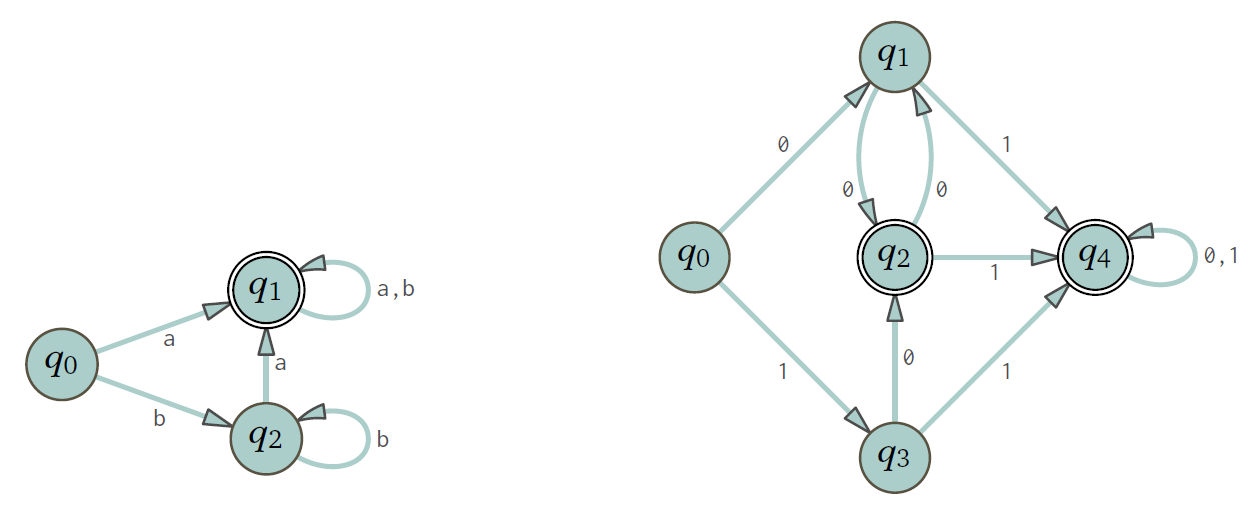
\includegraphics[width=0.75\textwidth]{Tarea 3 Enunciado 5.png}
            \label{Enunciado Ej. 5}
        \end{minipage}
    \item Apply to the same DFAs the algorithm seen in class.
    \item Explain intuitively why the algorithm works.
    \item Prove that the algorithm described obtains an equivalent DFA of minimum size.
\end{enumerate}

\clearpage

\subsection*{5.a}

We intend to apply the algorithm described in the exercise to the two given DFAs. The process goes as follows:

\textbf{First DFA:} This is the first DFA given.

\begin{figure}[h]
    \centering
    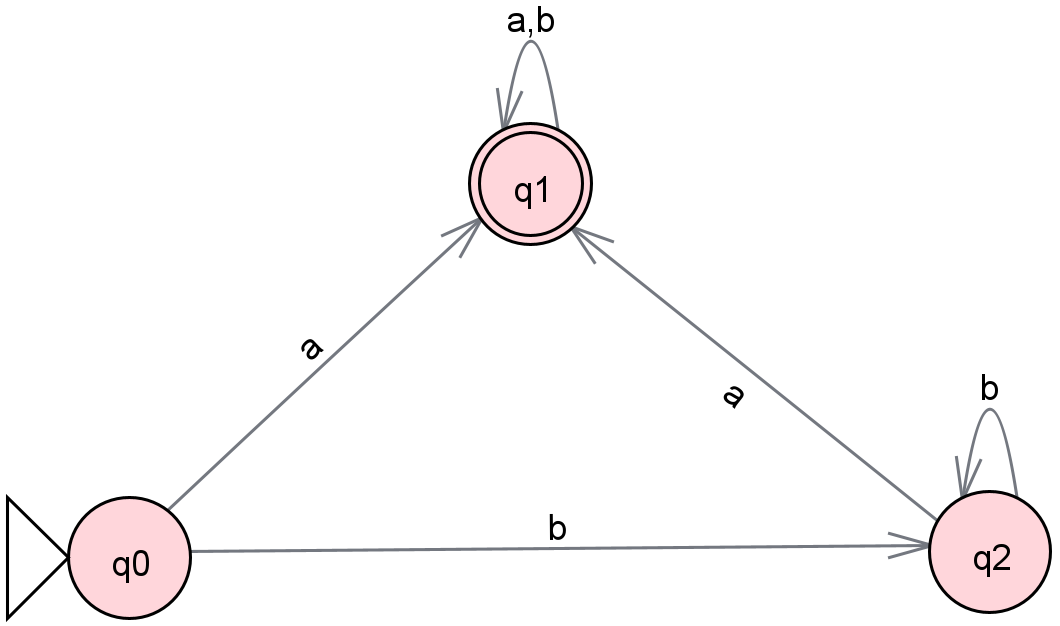
\includegraphics[width=0.7\linewidth]{First_Automaton.png}
\end{figure}

\textbf{Algorithm:}

\begin{enumerate}
    \item Construct the reverse NFA $M^R$ for $M$: To do this, reverse every transition (point every arrow backward, loops stay the same) and swap the roles of the starting and final states. Finally, as there may be multiple final states, we must create a starting state $s^R$ which takes to every final state in $M$ with $\varepsilon$-transitions.
\end{enumerate}


\begin{figure}[h]
    \centering
    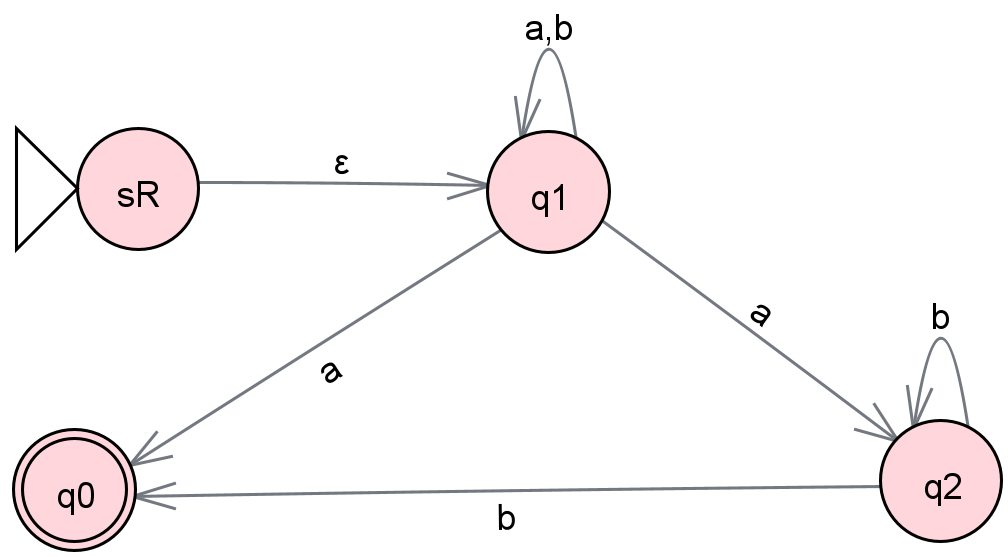
\includegraphics[width=0.7\linewidth]{First_Automaton_First_Step.png}
\end{figure}

\begin{enumerate}
    \setcounter{enumi}{1}
    \item Construct the DFA $\overline{M}$ equivalent to $M^R$: We now want to create a DFA from an NFA. For this purpose, we use the subset construction seen in class: The subset construction builds a DFA from an NFA in which the states are subsets of states in the NFA, and the transition function keeps track of all the states that can be reached from reading a symbol.
\end{enumerate}

\begin{figure}[h]
    \centering
    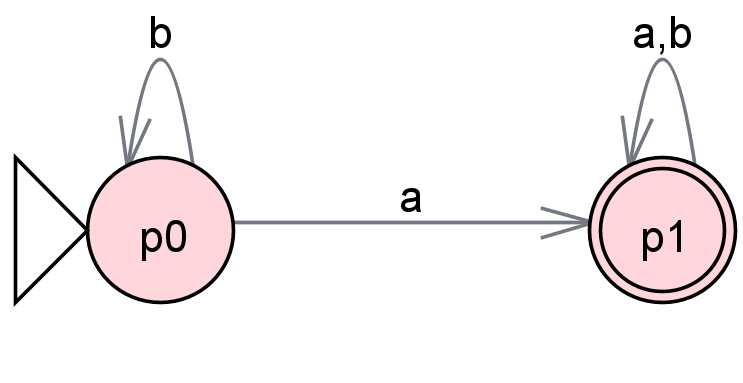
\includegraphics[width=0.7\linewidth]{First_Automaton_Second_Step.png}
\end{figure}

The following table shows the subset to which each state is corresponding:

\begin{center}
\begin{tabular}{|c|c|}
    \hline
    State & Corresponding subset of states in the NFA \\
    \hline
    $p0$ & $\{q1\}$ \\
    $p1$ & $\{q0, q1, q2\}$ \\
    \hline
\end{tabular}
\end{center}

\begin{enumerate}
    \setcounter{enumi}{2}
    \item Construct the reverse NFA $\overline{M^R}$ for $\overline{M}$: We repeat the process we did in step 1; we reverse every transition in the DFA and swap change final and initial states (remembering to add $s^R$). However, the states are the same as in step 2 (with adding $s^R$), and so, they represent the same subsets.

\begin{figure}[h]
        \centering
        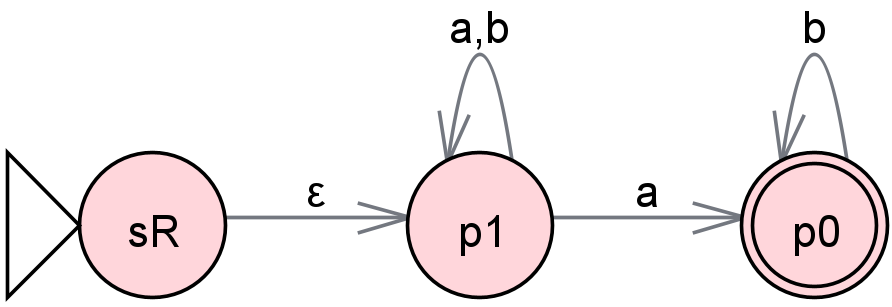
\includegraphics[width=0.7\linewidth]{First_Automaton_Third_Step.png}
\end{figure}
\bigskip\bigskip\bigskip\bigskip\bigskip\bigskip\bigskip\bigskip\bigskip

    \item Construct the DFA $\widehat{M}$ equivalent to $\overline{M^R}$: Once again, we repeat the process we did before. This time, the process we did in step 2. We want to create a DFA from the NFA in step 3 by using the subset construction.
    
\begin{figure}[h]
        \centering
        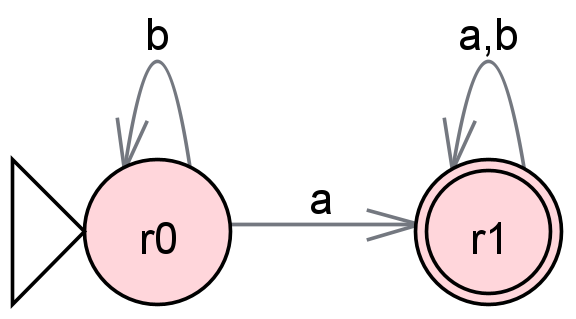
\includegraphics[width=0.5\linewidth]{First_Automaton_Fourth_Step.png}
\end{figure}

\end{enumerate}

The following table shows the subset to which each state is corresponding:

\begin{center}
\begin{tabular}{|c|c|}
    \hline
    State & Corresponding subset of states in the NFA \\
    \hline
    $r0$ & $\{p1\}$ \\
    $r1$ & $\{p0, p1\}$ \\
    \hline
\end{tabular}
\end{center}

\clearpage

\textbf{Second DFA:} The second DFA given.

\begin{figure}[h]
    \centering
    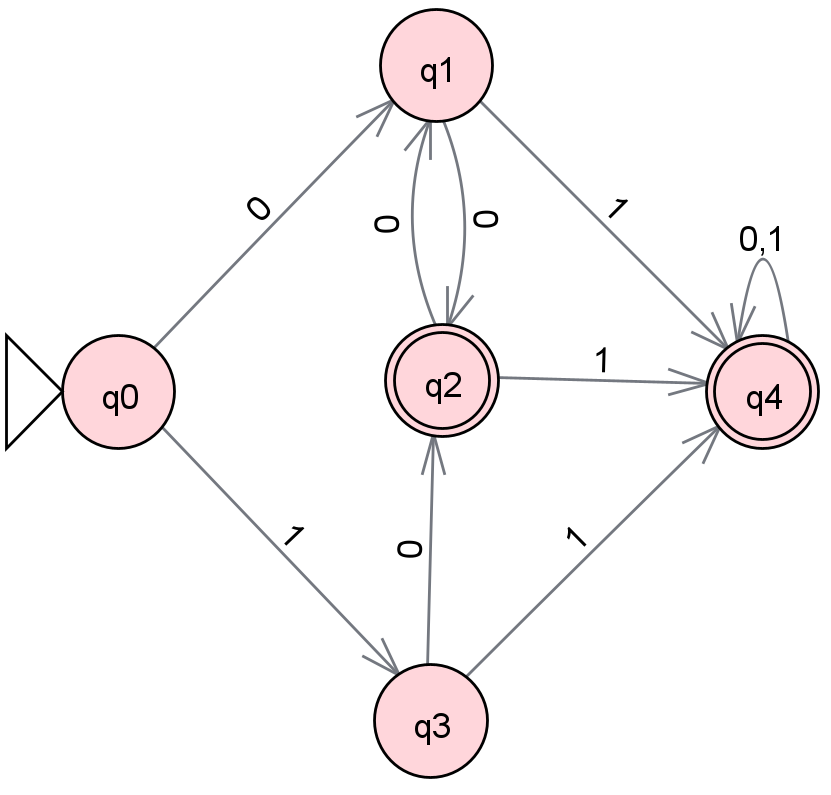
\includegraphics[width=0.5\linewidth]{Second_Automaton.png}
\end{figure}

\textbf{Algorithm:}

\begin{enumerate}
    \item Construct the reverse NFA $M^R$ for $M$: To do this, reverse every transition (point every arrow backward, loops stay the same) and swap the roles of the starting and final states. Finally, as there may be multiple final states, we must create a starting state $s^R$ which takes to every final state in $M$ with $\varepsilon$-transitions.

\begin{figure}[h]
    \centering
    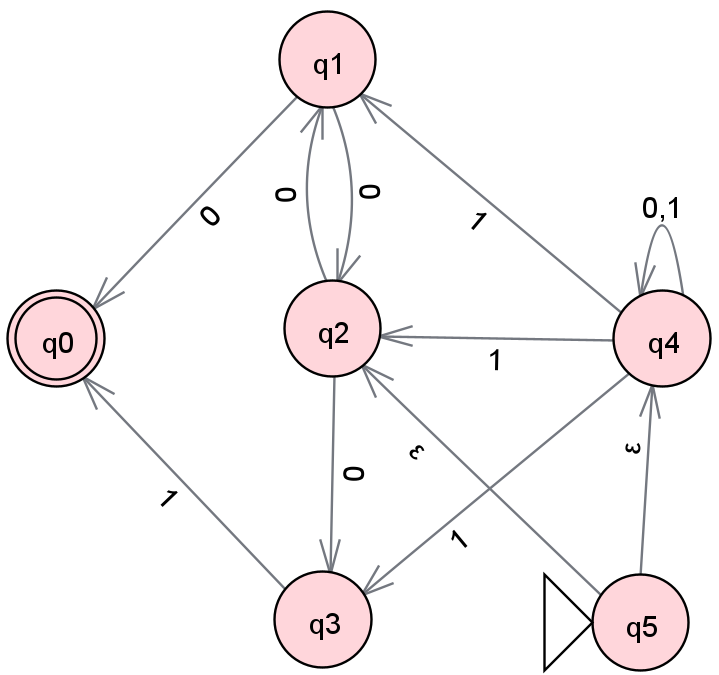
\includegraphics[width=0.5\linewidth]{Second_Automaton_First_Step.png}
\end{figure}
    
    \item Construct the DFA $\overline{M}$ equivalent to $M^R$: We now want to create a DFA from an NFA. For this purpose, we use the subset construction seen in class: The subset construction builds a DFA from an NFA in which the states are subsets of states in the NFA, and the transition function keeps track of all the states that can be reached from reading a symbol.

\begin{figure}[h]
    \centering
    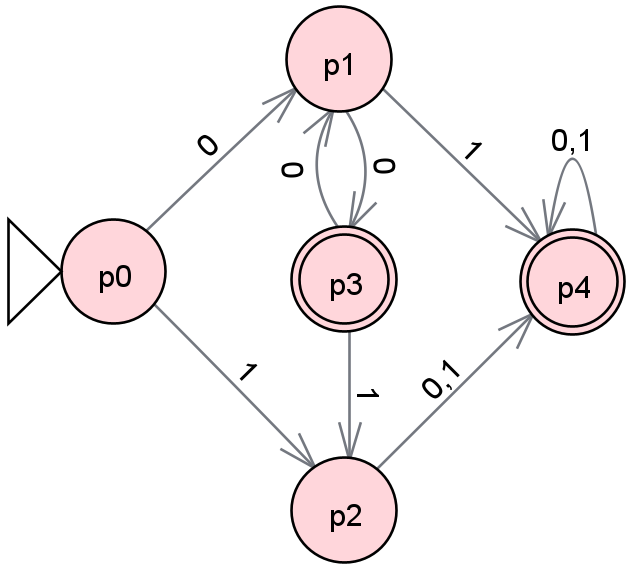
\includegraphics[width=0.5\linewidth]{Second_Automaton_Second_Step.png}
\end{figure}

\end{enumerate}

The following table shows the subset to which each state is corresponding:

\begin{center}
\begin{tabular}{|c|c|}
    \hline
    State & Corresponding subset of states in the NFA \\
    \hline
    $p0$ & $\{q2, q4\}$ \\
    $p1$ & $\{q1, q3, q4\}$ \\
    $p2$ & $\{q1, q2, q3, q4\}$ \\
    $p3$ & $\{q0, q2, q4\}$ \\
    $p4$ & $\{q0, q1, q2, q3, q4\}$ \\
    \hline
\end{tabular}
\end{center}

\begin{enumerate}
    \setcounter{enumi}{2}
    \item Construct the reverse NFA $\overline{M^R}$ for $\overline{M}$: We repeat the process we did in step 1; we reverse every transition in the DFA and swap change final and initial states (remembering to add $s^R$). However, the states are the same as in step 2 (with adding $s^R$), and so, they represent the same subsets.

\begin{figure}[h]
    \centering
    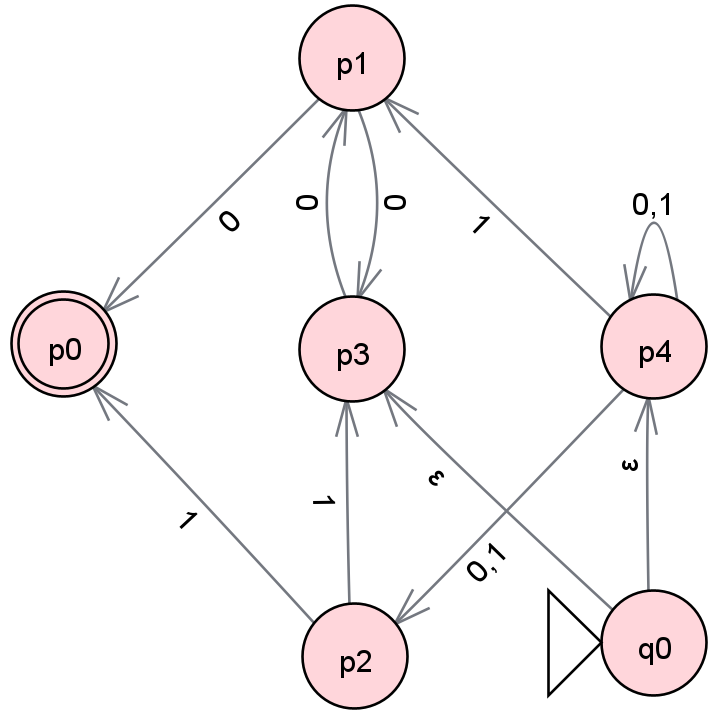
\includegraphics[width=0.5\linewidth]{Second_Automaton_Third_Step.png}
\end{figure}

\bigskip\bigskip\bigskip\bigskip\bigskip\bigskip\bigskip\

    \item Construct the DFA $\widehat{M}$ equivalent to $\overline{M^R}$: Once again, we repeat the process we did before. This time, the process we did in step 2. We want to create a DFA from the NFA in step 3 by using the subset construction.

\begin{figure}[h]
    \centering
    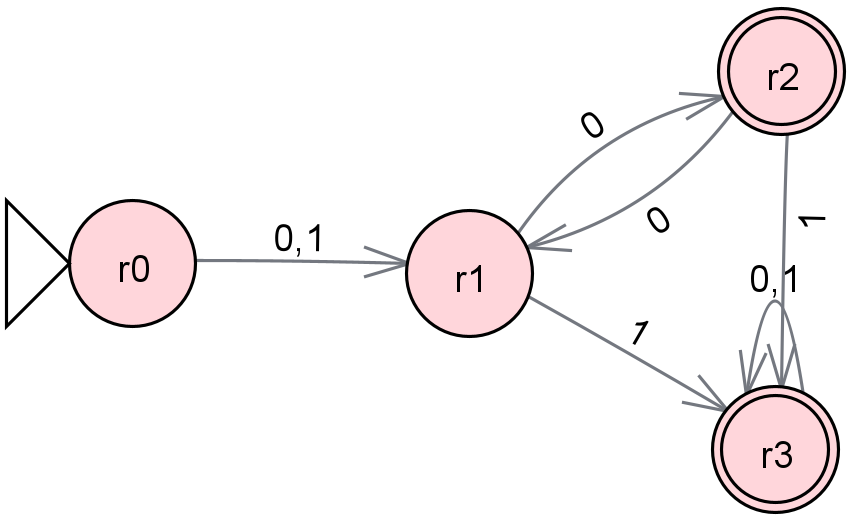
\includegraphics[width=0.5\linewidth]{Second_Automaton_Fourth_Step.png}
\end{figure}

\end{enumerate}

The following table shows the subset to which each state is corresponding:

\begin{center}
\begin{tabular}{|c|c|}
    \hline
    State & Corresponding subset of states in the NFA \\
    \hline
    $r0$ & $\{p3, p4\}$ \\
    $r1$ & $\{p1, p2, p4\}$ \\
    $r2$ & $\{p0, p2, p3, p4\}$ \\
    $r3$ & $\{p0, p1, p2, p3, p4\}$ \\
    \hline
\end{tabular}
\end{center}

\subsection*{5.b DFA Minimization Algorithm}

For this second part, we want to use the algorithm seen in class for DFA minimization. Briefly explained, this algorithm for DFA minimization completes the following steps: Consider an automaton with a number $n$ of states. Then,

\begin{enumerate}
    \item We construct a table of $n \times n$ where we number rows and columns with each of the states of the automaton. This table searches to mark which states are distinguishable.
    
    \item To then fill out the table, one must mark "X" wherever there is an integer number $k$ where $p \not\equiv_k q$, where $p, q \in Q$, the set of the states of the automaton. That is, if there is a string of length $k$ that distinguishes $p$ and $q$.
    
    \item Finally, after reaching a $k$ where it no longer yields results (this $k$ is, intuitively, the minimal number of transitions to take from the initial state to each final state), you must check the table for which states are then indistinguishable. Those states

 may be "collapsed" into each other, making a single state that has the same suffix language, and that, therefore, does not change the language that the automaton accepts.
\end{enumerate}

\textbf{Important Note:} First, note that no matter what, there is no way to distinguish one state from itself. Therefore, the main diagonal of the table will never have X's. Following that, note that $\equiv_k$ is an equivalence relationship. For that reason, it must be reflexive. Therefore, if the index $ij$ of the table is marked with an X, then so must be the index $ji$. That is all to say that you do not need to make or fill the entire table; it is just necessary to check all the boxes in the superior or lower triangle left after dividing the table by the diagonal. Check the following examples for clarification.

\bigskip\bigskip\bigskip\bigskip\bigskip\bigskip\bigskip\bigskip\bigskip\bigskip\bigskip\bigskip\bigskip\bigskip\bigskip

\textbf{First DFA:}

\begin{figure}[h]
    \centering
    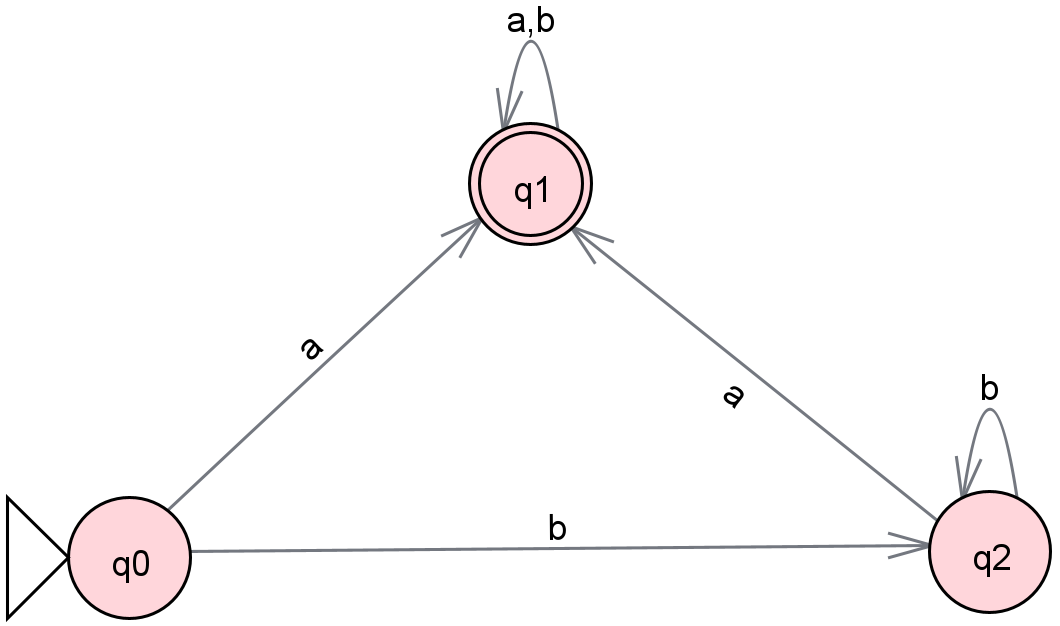
\includegraphics[width=0.7\linewidth]{First_Automaton.png}
\end{figure}

We then fill out the following table: The boxes in pink are not necessary to fill out (see the Important Note).

\begin{center}
\begin{tabular}{|c|c|c|c|}
    \hline
    & $q0$ & $q1$ & $q2$ \\
    \hline
    $q0$ &\cellcolor{pink!50}&\cellcolor{pink!50}&\cellcolor{pink!50} \\
    $q1$ & X &\cellcolor{pink!50} &\cellcolor{pink!50} \\
    $q2$ & & X &\cellcolor{pink!50} \\
    \hline
\end{tabular}
\end{center}

Let's detail why each box is marked:
\begin{itemize}
    \item $(q0, q1)$: $\varepsilon$ distinguishes them. $k=0$
    \item $(q1, q2)$: $\varepsilon$ distinguishes them. $k=0$
\end{itemize}

See that $(q0, q2)$ isn't marked. That's because $q0 \equiv_2 q2$, that is, for any string $z \in \{a, b\}^*$ such that $|z| \leq 2$, $\delta(q0, z) \in F \iff \delta(q2, z) \in F$. Formally, we could check algorithmically:

\begin{itemize}
    \item For $z=a$: $\delta(q0, z) \in F$ and $\delta(q2, z) \in F$
    \item For $z=b$: $\delta(q0, z) \not\in F$ and $\delta(q2, z) \not\in F$
    \item For $z=aa$: $\delta(q0, z) \in F$ and $\delta(q2, z) \in F$
    \item For $z=ab$: $\delta(q0, z) \in F$ and $\delta(q2, z) \in F$
    \item For $z=ba$: $\delta(q0, z) \in F$ and $\delta(q2, z) \in F$
    \item For $z=bb$: $\delta(q0, z) \not\in F$ and $\delta(q2, z) \not\in F$
\end{itemize}

(Take into account this might not be viable in other scenarios). We've proven that $q0$ and $q2$ are indistinguishable. We then proceed to "collapse" them into the same state. The resulting automaton is the following:

\begin{figure}[h]
        \centering
        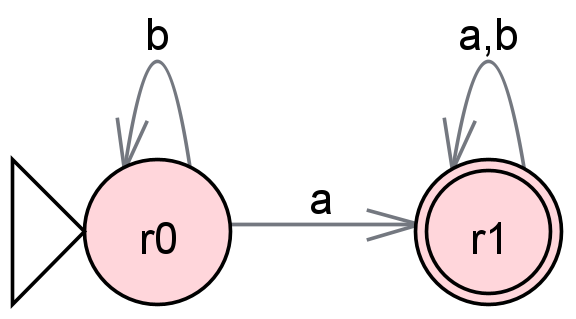
\includegraphics[width=0.4\linewidth]{First_Automaton_Fourth_Step.png}
\end{figure}

Where:

\begin{center}
\begin{tabular}{|c|c|}
    \hline
    State & Corresponding States in the Automaton \\
    \hline
    $r0$ & $\{q0,q2\}$ \\
    $r1$ & $\{q1\}$ \\
    \hline
\end{tabular}
\end{center}

\textbf{Second DFA:}

\begin{figure}[h]
    \centering
    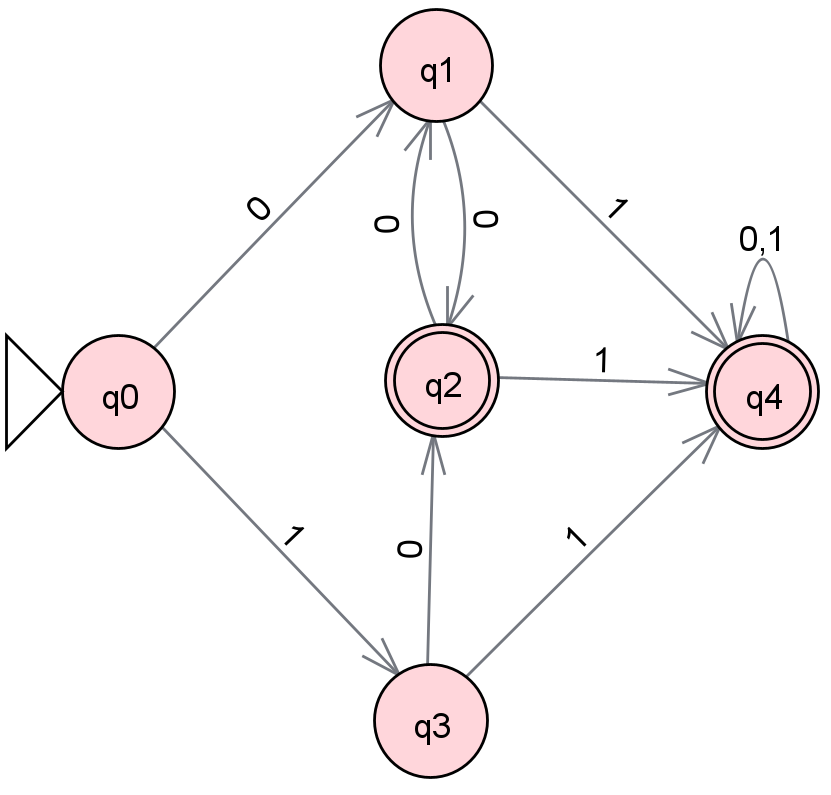
\includegraphics[width=0.5\linewidth]{Second_Automaton.png}
\end{figure}

We then fill out the following table: The boxes in pink are not necessary to fill out (see the Important Note).

\begin{center}
\begin{tabular}{|c|c|c|c|c|c|}
    \hline
    & $q0$ & $q1$ & $q2$ & $q3$ & $q4$\\
    \hline
    $q0$ &\cellcolor{pink!50}&\cellcolor{pink!50}&\cellcolor{pink!50}&\cellcolor{pink!50}&\cellcolor{pink!50} \\
    $q1$ & X &\cellcolor{pink!50}&\cellcolor{pink!50}&\cellcolor{pink!50}&\cellcolor{pink!50} \\
    $q2$ & X & X &\cellcolor{pink!50}&\cellcolor{pink!50}&\cellcolor{pink!50} \\
    $q3$ & X & & X &\cellcolor{pink!50}&\cellcolor{pink!50} \\
    $q4$ & X & X & X & X &\cellcolor{pink!50} \\
    \hline
\end{tabular}
\end{center}

Let's detail why each box is marked:

\begin{itemize}
    \item $(q0, q2)$: $\varepsilon$ distinguishes them. $k=0$
    \item $(q0, q4)$: $\varepsilon$ distinguishes them. $k=0$
    \item $(q1, q2)$: $\varepsilon$ distinguishes them. $k=0$
    \item $(q1, q4)$: $\varepsilon$ distinguishes them. $k=0$
    \item $(q2, q3)$: $\varepsilon$ distinguishes them. $k=0$
    \item $(q3, q4)$: $\varepsilon$ distinguishes them. $k=0$
    \item $(q0, q1)$: 1 distinguishes them. $k=1$
    \item $(q0, q3)$: 1 distinguishes them. $k=1$
    \item $(q2, q4)$: 0 distinguishes them. $k=1$
\end{itemize}

See that $(q1, q3)$ isn't marked. That's because $q1 \equiv_M q3$, that is, for any string $z \in \{a, b\}^*$, $\delta(q1, z) \in F \iff \delta(q3, z) \in F$. It isn't viable to check it algorithmically by ourselves (since we explained before that we should at least try with a $k$ of at least the number of transitions needed to get from the initial state to a final state, and that would mean to try $2^{1+2^2+2^3}$ strings, which isn't practical!). We can, however, try to see it intuitively. See that, from $q0$ and $q1$, any string that contains a singular 1 will take to a final state, and any amount of 0s and 1s after that will still end up in a final state. But also notice, both states with a singular 0 take to a final state, but with 00 they do not take to a final state. In fact, in that case, they both end up in state $q1$, and after that, any odd amount of 0s will result in a final state, whereas any string of 0s of even length will take back again to $q1$ (not a final state). In any case, $q1 \equiv_M q3$, which means that we can "collapse" $q1$ and $q3$ into a singular state and, therefore, minimize the DFA.

\bigskip\bigskip\bigskip\bigskip\bigskip\bigskip\bigskip\bigskip\bigskip\bigskip\bigskip\bigskip\bigskip\bigskip\bigskip

The resulting automaton is as follows:

\begin{figure}[h]
    \centering
    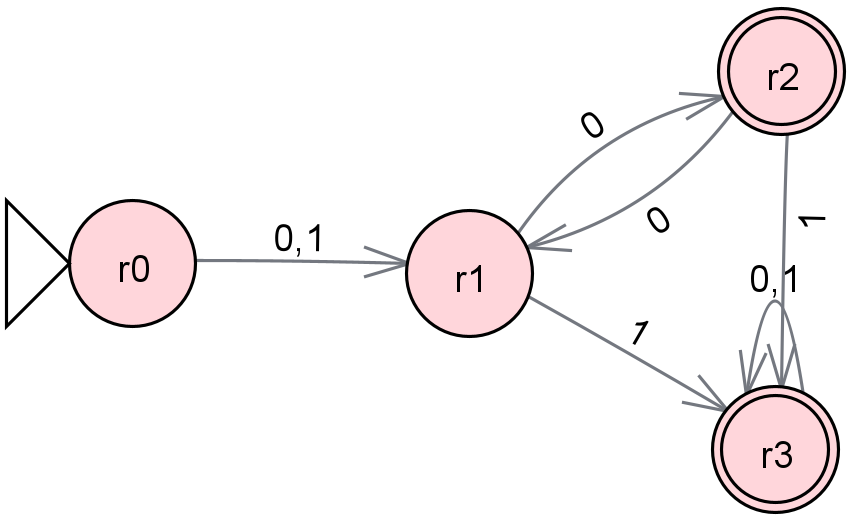
\includegraphics[width=0.5\linewidth]{Second_Automaton_Fourth_Step.png}
\end{figure}

Where:

\begin{center}
\begin{tabular}{|c|c|}
    \hline
    State & Corresponding States in the Automaton \\
    \hline
    $r0$ & $\{q0\}$ \\
    $r1$ & $\{q1, q3\}$ \\
    $r2$ & $\{q2\}$ \\
    $r3$ & $\{q4\}$ \\
    \hline
\end{tabular}
\end{center}


\subsection*{5.c Explanation of Algorithm}

There is an intuitive idea of why this new algorithm alternative works and outputs a minimized DFA. The key to why this works is in the reversal process, the subset construction, and the number of steps.

\begin{enumerate}
    \item First step: The first step of this process consists of putting the given automaton that you wish to minimize through a reversal process, which is the one shown in the description of the problem. The reason why we're reversing the automaton is essential: We're putting into the language of automatons the definition of suffix languages. In class, we defined the equivalence relation $\equiv_N$ as: For $p, q \in Q$, $p \equiv_N q$ if $L_p^S = L_q^S$. In simpler words, we're identifying which states take to final states with the same set of strings. However, if you're clever enough (or if you actually read the notes), you might have noticed that any states that are $\equiv_N$ are "collapsed" into each other whenever we used the algorithm for DFA minimization we explained in class as well. This is because both states are "redundant" in the sense that, whenever we reach those states, we can use the same string to get to a final state, and therefore, there might be a way to merge them into a state that will be reached by a "union" of the prefix languages and will have the same suffix language. In automatons, since neither a DFA nor an NFA can read the input string backward, there is no way to check (mathematically, or rather, computationally) for the suffix language of each state to see if it is necessary to collapse certain states that have the same suffix language. For this purpose, we reverse the transitions, and now, we have an automaton that goes from the final states to the initial state. If we analyzed the prefix languages of this reversed automaton, we would get the suffix languages of the states in the non-reversed one. And just like that, we got a key piece of information that is mandatory to know which states will be collapsed into each other clearly from an automaton (and not from intuition or from "seeing the graph").
    
    \item Second step: This step is one of the most important for this process (although it obviously needs the others to be complete and correct) for the sole reason that here is where one part of the minimization of the automaton happens. This step involves using the subset construction of a DFA from an NFA that was explained in class. The subset construction consists of making each of the states of the new DFA a subset of the states in the NFA and make transitions according to which subset of states will take a transition from each subset. In other words, if the NFA could reach a few different states with one input from the starting state, then we would make a state for the starting state in the DFA and make a transition with said symbol to another state that represents the subset of states that are reachable by reading that symbol. The reversed automaton we got from the first step is, again, an NFA, meaning, we can use the subset construction to make an equivalent DFA. Following the process, we want to make a new set of states that are subsets of the states in the reversed automaton. However, and here comes the magic, notice that:
    
    \begin{itemize}
        \item First, the initial states of the reversed automaton are the final states of the original one.
        \item Second, the transitions that go "out" from these new initial states are the transitions that go "in" in the original automaton.
        \item Then, if there are two or more states that, by reading a symbol a, get to a final state, then in the reversed automaton, from that final state, we may reach by reading a the states that lead to it in the original automaton.
        \item And, in the subset construction from the reversed automaton, since there are two or more states that can be reached from reading the same input from a state, then they may be merged into a new state in the new DFA (which will represent that subset of states).
    \end{itemize}
    
    And, voilà. Just like that, we've explained (just in words) how the automaton gets minimized (although partially). Notice how if two states go to a final state with the same subset of strings, then they may be reached with that same subset of strings from the final state in the reversed automaton. And, since they may both be reached with the same transitions, we can merge them into the same state in the new DFA we're constructing. For this step, we can assure that states that have the same suffix language are merged. There is a slight issue, however, this DFA is backward,
    
    \item To solve this slight (not slight at all) issue, we do the third and fourth steps, which are, essentially, the re-reversing process. The third step is, again, reversing the automaton that we just created, since the one we have accepts $L^R$, and we need one that accepts $L$. We proceed to reverse it, and as the problem pointed out, after we've applied the process on the DFA of the second step, the resulting automaton from this process is not a DFA, but rather, an NFA. This is also an issue.
    
    \item For this issue, we have the fourth step. Again, this step is practically equal to the second step (and there is no need to explain it here again), and again, it outputs a DFA, which is the DFA that accepts the same language that the reversed automaton of step 3 accepts. We notice that if two states could be reached with the same transitions from the same state in the reversed automaton, then they could reach a singular state in the automaton in the third step (although they may not have the same suffix language). We can also notice that we only needed to perform the steps 2, 3, and 4 for the reversed automaton, since, the other one, which is constructed in step 1, will contain all the necessary information (the suffix languages and the steps) to see if two states in it are indistinguishable, or if they will be merged when applying the algorithm we saw in class (for DFA minimization).
\end{enumerate}

\subsection*{5.d Proof Idea}

For this demonstration, we will follow the construction outlined in the problem. Specifically, we must:

\begin{enumerate}
    \item Start with any automaton $M = (Q, \Sigma, \delta, q_0, F)$.
    \item Construct $M^R$ from $M$ using the procedure specified in the problem.
    \item From $M^R$, construct $\overline{M}$, the equivalent DFA of $M^R$, using the subset construction.
\end{enumerate}

Clearly, $\overline{M}$ accepts $L^R$, but we need it to accept $L$ instead. 

\begin{enumerate}
    \setcounter{enumi}{3}
    \item Then, construct $\overline{M}^R$ from $\overline{M}$ using the reversing process described in the problem.
    \item Finally, since $\overline{M}^R$ is an NFA, construct $\widehat{M}$, an equivalent DFA, using the subset construction.
\end{enumerate}

It is essential to take into account that the demonstration will be based on these constructions. After constructing $\widehat{M}$, we must demonstrate that it is minimal. Therefore, we must assume that our starting automaton $M$ had a regular language $L$, and based on that, we can construct $M_O$, the minimized DFA for $L$. Finally (and probably the most challenging part), we must show that $\widehat{M}$ and $M_O$ are equivalent. If we can prove this, we demonstrate that $\widehat{M}$ is minimal, as DFAs of minimum size for a regular language are unique up to isomorphism.

\subsubsection*{(Attempt of) Proof}

Suppose a DFA $M = (Q, \Sigma, \delta, q_0, F)$ that accepts a language $L$. We construct $M^R = (Q^R, \Sigma, \delta^R, q_0^R, F^R)$, the reverse automaton of $M$, where:

\begin{align*}
    Q^R &= Q \cup \{q_0^R\} \\
    F^R &= \{q_0\} \\
    \delta^R(s^R, \varepsilon) &= F \\
    \delta^R(s^R, a) &= \emptyset, \quad \forall a \in \Sigma \\
    \delta^R(q, \varepsilon) &= \emptyset, \quad \forall q \in Q \\
    \delta^R(q, a) &= \{p \,|\, q \in \delta(p, a)\}, \quad \forall q \in Q, \, \forall a \in \Sigma
\end{align*}

I’m stuck! Don’t know how to define the subset construction mathematically :p. 

\end{document}
